\documentclass[a4paper]{book}
\usepackage[utf8]{inputenc}
\usepackage[hidelinks]{hyperref}
\usepackage{pdfpages}
\usepackage{fullpage}
\usepackage{fancyhdr}
\usepackage{xcolor}
\usepackage{graphicx}
\usepackage{wrapfig}
\usepackage{baskervald}
\usepackage{geometry}
\usepackage{multicol}
\fancyhead{}
\fancyfoot[LE,RO]{\thepage}
\cfoot{}
\fancyfoot[LO,RE]{The miniKanren and Relational Programming Workshop 2023}
\renewcommand{\headrulewidth}{0.0pt}
\date{September 8, 2023}
\author{Nada Amin \and William E. Byrd}
\begin{document}
\frontmatter
\setcounter{page}{3}  % cover page to be added by TR editor
\newgeometry{textheight=8.5in,hmargin=20mm}
\chapter*{Preface}
This report aggregates the papers presented at the fifth miniKanren
and Relational Programming Workshop, hosted on September 8, 2023 in
Seattle, WA, USA and co-located with the twenty-eight International
Conference on Functional Programming.

\vspace{5pt}
\noindent
The miniKanren and Relational Programming Workshop is a workshop for the miniKanren family of relational (pure constraint logic programming) languages: miniKanren, microKanren, core.logic, OCanren, Guanxi, etc. The workshop solicits papers and talks on the design, implementation, and application of miniKanren-like languages. A major goal of the workshop is to bring together researchers, implementors, and users from the miniKanren community, and to share expertise and techniques for relational programming. Another goal for the workshop is to push the state of the art of relational programming—for example, by developing new techniques for writing interpreters, type inferencers, theorem provers, abstract interpreters, CAD tools, and other interesting programs as relations, which are capable of being “run backwards,” performing synthesis, etc.

\vspace{5pt}
\noindent
Five papers were submitted to the workshop, and each submission was reviewed by
two to three members of the program committee.  After deliberation, four submissions were accepted to the workshop.

\vspace{5pt}
\noindent
In addition to the four full papers presented
\begin{itemize}
\item William E. Byrd gave a morning tutorial on miniKanren,
\item the workshop closed with an open discussion on the future of miniKanren.
\end{itemize}

\vspace{5pt}
\noindent
Thanks to all presenters, participants, and members of the
program committee.

\ \\

\ \ \ \ \ \ \ Nada Amin \& William E. Byrd

\ \\

\section*{Program Committee}
\noindent
Nada Amin, Harvard University, USA (Co-Chair)\\
Michael Arntzenius, RelationalAI, UK\\
Oliver Bračevac, Galois, Inc., USA\\
William E. Byrd, University of Alabama at Birmingham, USA (Co-Chair)\\
Evan Donahue, University of Tokyo, Japan\\
Thomas Gilray, University of Alabama at Birmingham, USA\\
Ekaterina Komendantskaya, Heriot-Watt University and Southampton University, UK\\
Ekaterina Verbitskaia, JetBrains, Serbia\\

\tableofcontents
\mainmatter
\newgeometry{textheight=9.5in,hmargin=20mm}

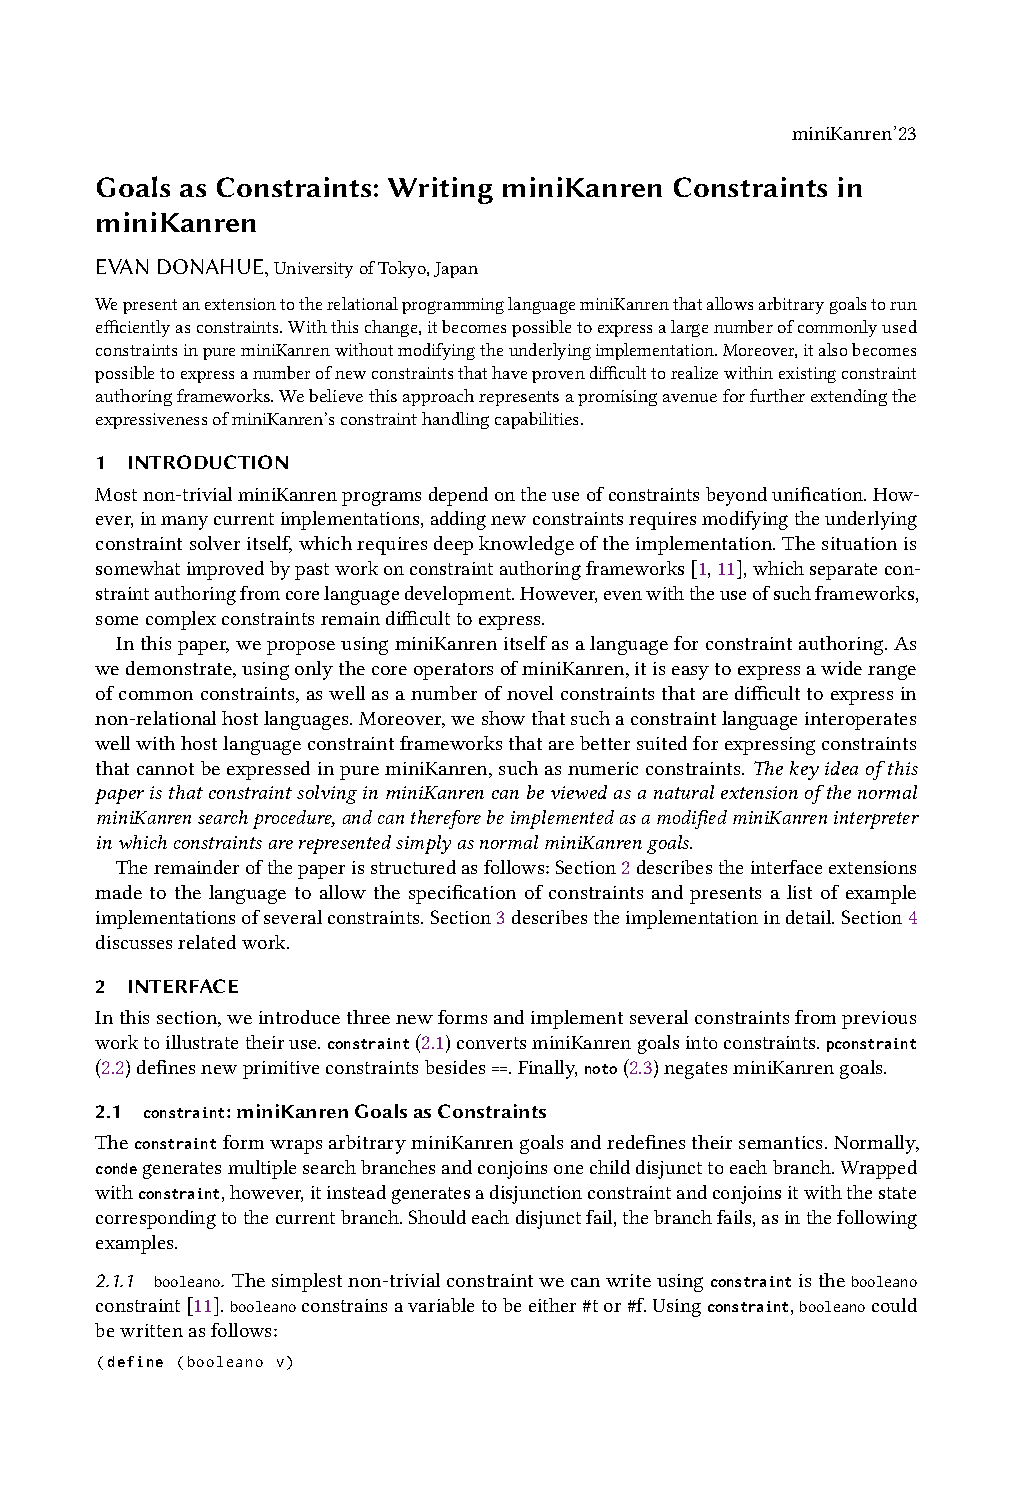
\includepdf[noautoscale,scale=1.07,pages=-,pagecommand={\thispagestyle{fancy}},addtotoc={1,chapter,1,{Goals as Constraints: Writing miniKanren Constraints in miniKanren by Donahue},p1}]{minikanren23-final1}

\ \\
\pagebreak

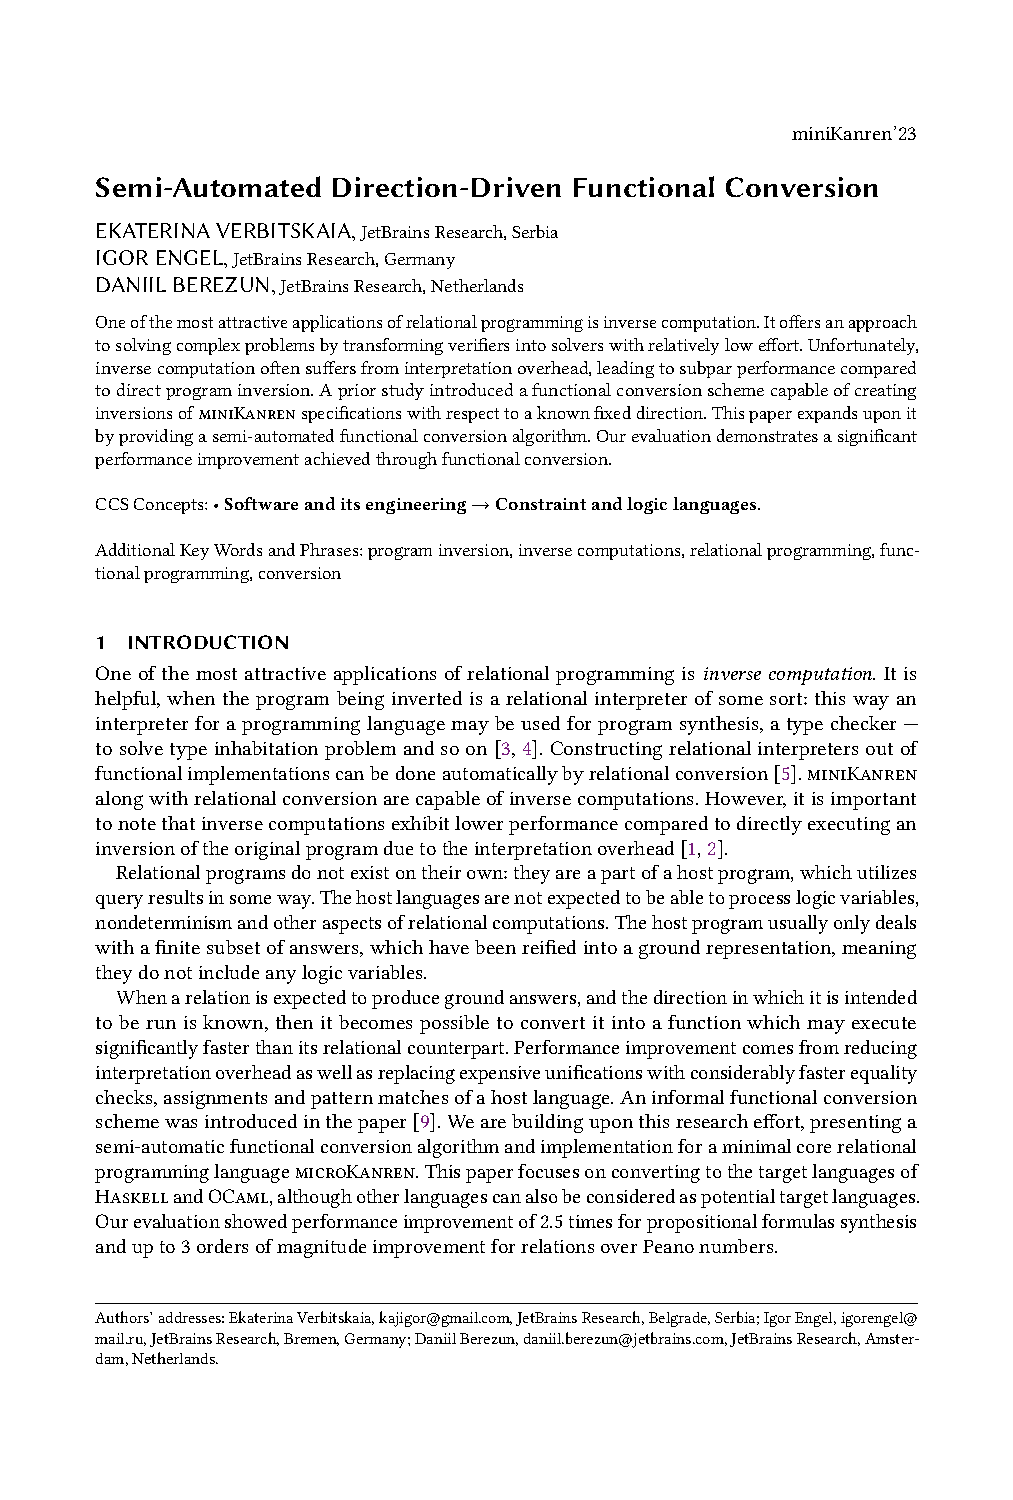
\includepdf[noautoscale,scale=1.07,pages=-,pagecommand={\thispagestyle{fancy}},addtotoc={1,chapter,2,{Semi-Automated Direction-Driven Functional Conversion by Verbitskaia, Engel \& Berezun},p2}]{minikanren23-final2}

\ \\
\pagebreak

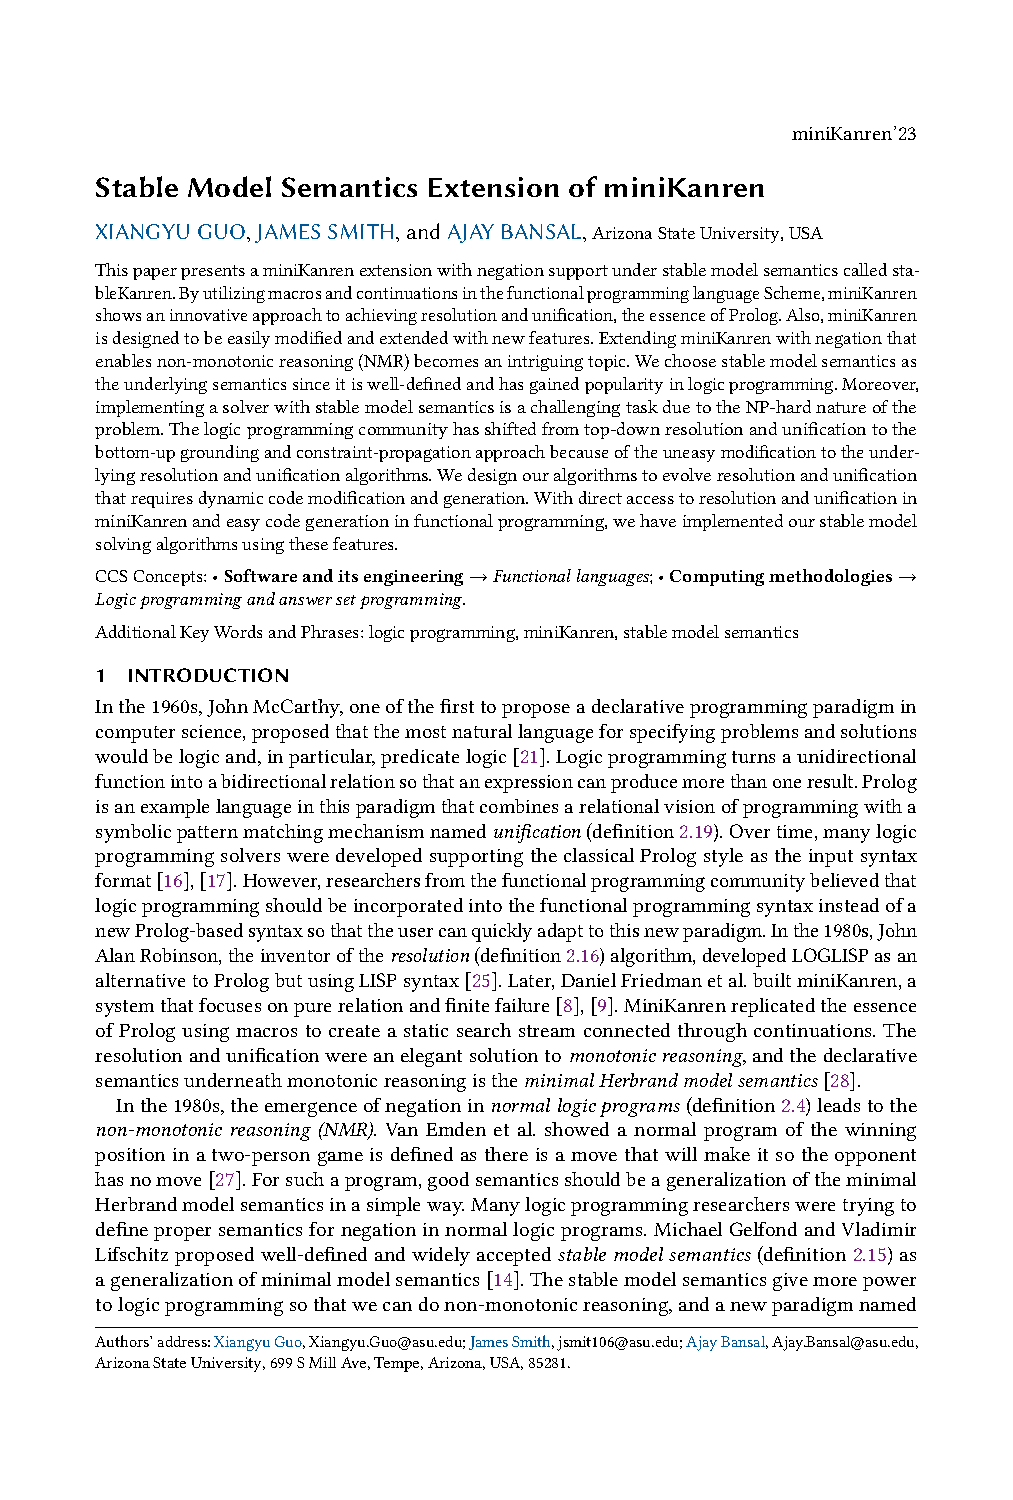
\includepdf[noautoscale,scale=1.07,pages=-,pagecommand={\thispagestyle{fancy}},addtotoc={1,chapter,3,{Stable Model Semantics Extension of miniKanren by Guo, Smith \& Bansal},p3}]{minikanren23-final3}

\ \\
\pagebreak

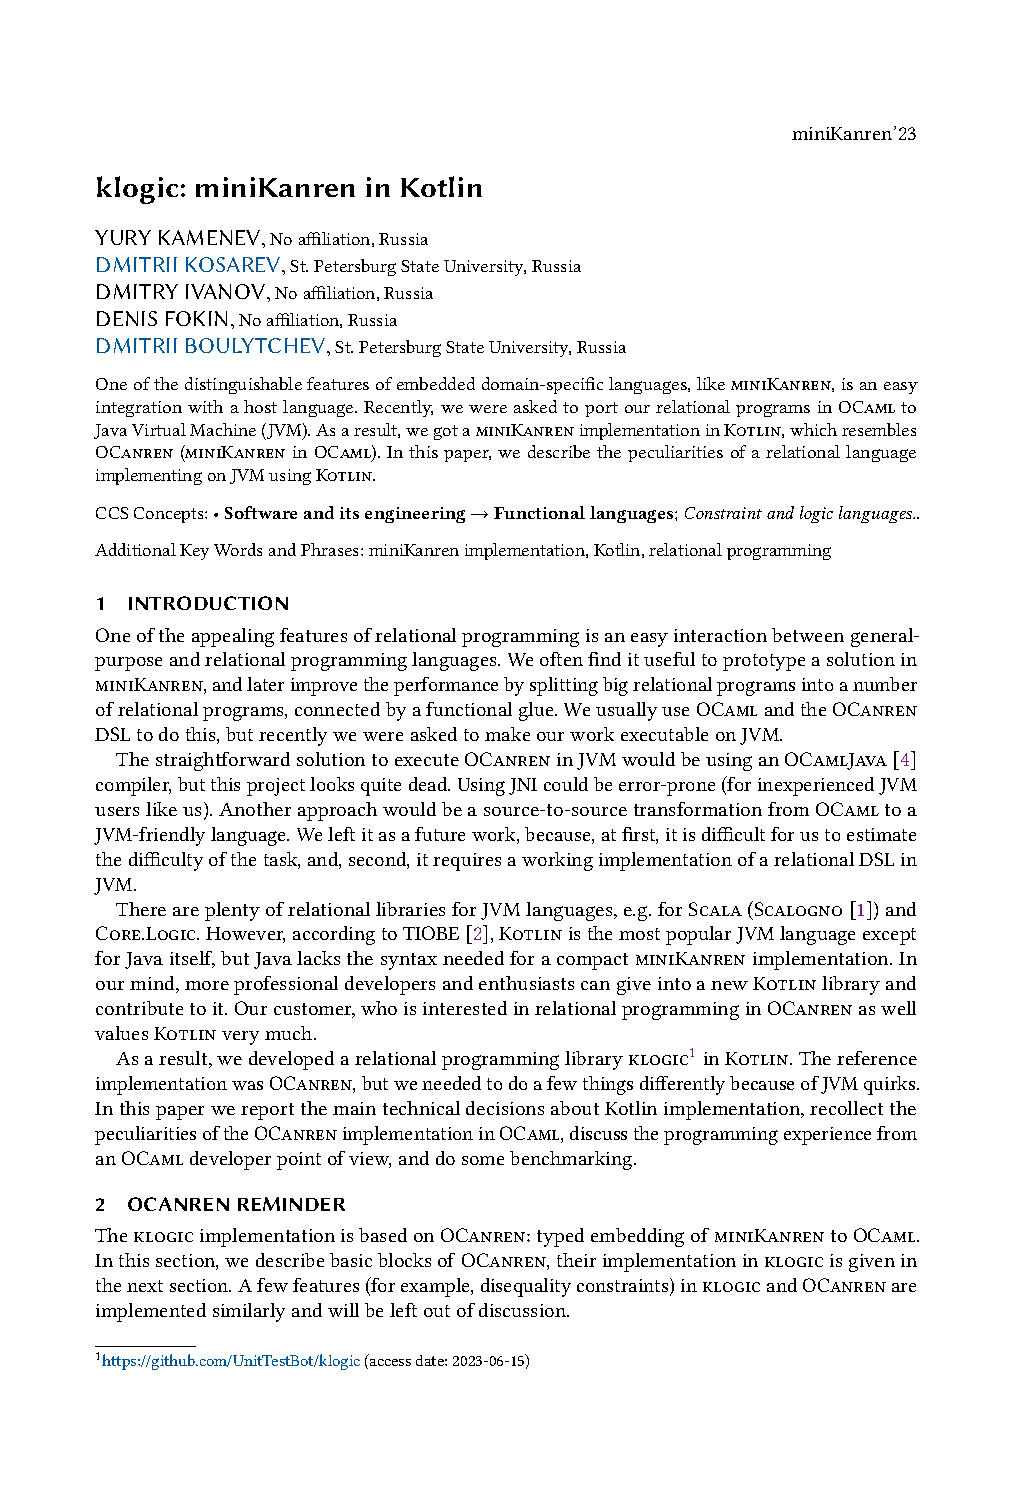
\includepdf[noautoscale,scale=1.07,pages=-,pagecommand={\thispagestyle{fancy}},addtotoc={1,chapter,4,{klogic: miniKanren in Kotlin by Kamenev, Kosarev, Ivanov, Fokin \& Boulytchev},p4}]{minikanren23-final4}

\ \\
\pagebreak

\end{document}
